% Chapter Template

\chapter{Introduction} % Main chapter title

\label{chapter-introduction} % Change X to a consecutive number; for referencing this chapter elsewhere, use \ref{ChapterX}

\lhead{Chapter . \emph{Introduction}} % Change X to a consecutive number; this is for the header on each page - perhaps a shortened title

%----------------------------------------------------------------------------------------
%	SECTION 1
%----------------------------------------------------------------------------------------

In the current days robots are starting to be introduced in our lives more and more, and we can expect that, in the next years, they will complete the transition from mechanic tools, used mostly in industries, to true partners and companions. There is an increasing interest in studying how robots should behave in environments inhabited by humans, and in some works robots have been deployed in crowded and dynamic environments, like airports and museums.

Human-Robot cooperation poses a multitude of problems. Imagine a mobile robot working in a warehouse, carrying and sorting crates in different locations. Already, we are presented with quite a complex problem, where the robot needs to have a good representation of the world (i.e. position of the crates, obstacles, layout of the warehouse), to create plans to reach the goal (which crates to move, where to bring them, which paths to follow), and to have sufficient motion and manipulation skills to achieve them. If humans are present in the environment, they should be represented and considered by the robot in its plans and actions.  Modeling humans as simple moving obstacles might not be enough if we consider issues of trust, legibility, and acceptability. The robot should respect a number of social rules in the presence of humans, like maintaining a socially acceptable distance, whenever possible, from them, and approaching them from a visible positions.

The problem becomes even more complex when robots and humans need to cooperate to solve a goal, for example by sorting together the crates, or even by sharing the load of heavy objects. To understand  how to approach this problem we can observe how humans cooperate with themselves. Psychological and philosofical research \cite{pacherie2012phenomenology} characterizes the execution of cooperative actions as 'joint actions'. Sebanz et al. \cite{sebanz2006joint} have proposed that the execution of a joint action depends on three different abilities: sharing representations, predicting actions, and integrating predicted effects of own and other's actions. These abilities can be achieved by the combination of different mechanisms:
\begin{itemize}
\item Joint Attention. The ability to direct a partner's attention, in order to create a shared representation of objects and events. Humans use a large number of social cues, like gaze direction or pointing gestures, to indicate what is currently under observation. This mechanism helps filling important gaps in the knowledge of a partner, and points to the importance of understanding what others know and perceive.
\item Action Observation: observing other partners' actions is crucial in understanding what are their goals. Studies have shown that observing a person performing an action produces a motor resonance, which increases with the observer's level of expertise in the action. Understanding what others are doing allows to predict the outcomes of their activities, and even their next movements.
\item Task Sharing: humans are able to predict, in some circumstances, what others will do  even without direct observation. A notable example is a well trained sport team, which is able to act like a single entity, coordinating seamlessly. This ability suggests that humans possess a shared representation of tasks, which include actions that should be performed by each partner of the team.
\item Action Coordination: predicting actions is not enough. Humans also need to choose a complementary action, and adjusting its parameters, like the exact moment and place where it should be performed, to partners. 
\end{itemize}

It seems that robots need to have an equivalent of these mechanism, in order to cooperate in a natural and acceptable way with humans. Is this enough to include robots in our lives? Unfortunately, we just scratched the surface of the problem. While these areas are already very complex, and not completely understood, humans possess other skills, that should be translated to robots. For example, when a robot's behavior shows a degree of intelligence, humans usually try to have a conversation with it, which can lead to frustation, or often disbelief in the actual capacities of the robot. Issues such as dialogue, representation and refinement of knowledge are very complex and will be a direct focus of this work.

The goal of this thesis is, instead, to provide a framework to allow a robot to work in social environments and execute joint actions with humans in a natural way. We built our system using psychology as an inspiration, without trying to replicate accurately human mechanism, an area of work studied in cognitive systems. 

There are still not many robotic architecture that take humans into account at all levels, from planifications to execution. We will review some examples:
\begin{itemize} 
\item \cite{trafton2013act} presents ACT-R/E, a cognitive architecture, based
on the ACT-R architecture, used for human robot interaction tasks. The
architecture aims at simulating how humans think, perceive and act in
the world. ACT-R/E has being tested in different scenarios, such as
theory of mind and hide and seek, to show its capacity of modeling
human behaviors and tought.
\item In \cite{Fong_2006} the authors present  HRI/OS, an agent-based system
that allows humans and robots to work in teams. The system is able to
produce and schedule tasks to different agents, based on their capacities,
and allows the agents to interact mostly in a parallel and independent way, with
loose coordination between them. Cooperation  mainly
takes place when one agent asks for help while
dealing with a situation. In this case the HRI/OS will
look for the best agent to help, based on their availability and capacities.

\item In \cite{clodic2009shary} the authors build SHARY, a supervision
system for human robot interaction, tested in domestic environments to
perform tasks such as serving a drink to a person. Our system is an
evolution of Shary which includes new aspects, like spatial
reasoning and modeling of joint actions.
\end{itemize}

\section{Contributions}

The main contributions of this work are the following:
\begin{itemize}
\item Building a supervision system for human robot interaction, integrating novel algorithms developed in this work with existing, components.
\item Developing a novel algorithm to infer human goals and intentions.
\item Developing a novel probabilistic planning algorithm for multiple agent.
\end{itemize}

\section{System overview}
\label{intro-system_overview}
%TODO: add urls, PR2, GAZEBO, ROS, SPENCER, GTP, Move_Base, Moveit
The supervision system was developed with the following goals:
\begin{itemize}
\item Flexibility. The system is able to work in different scenarios, environments, and different robots.
\item Extendibility. The system can be easily extendable by adding or substituting modules, to introduce different capacities, without having an impact on existing components.
\item Human-Awareness. The system supports human in all its layers. Human belief management, multi-agent planning, human-aware motion and execution, and simple forms of direct interaction are explicitly included in its components.
\end{itemize}

To achieve these goals we use the well-known ROS framework\footnote{http://www.ros.org/}, which naturally supports different robots and modules.The system has been implemented and tested in simulation, using the GAZEBO simulator\footnote{http://gazebosim.org/}, and on two different robots, the PR2 by Willow Garage\footnote{https://www.willowgarage.com/pages/pr2/overview}, and the SPENCER robot\footnote{http://www.spencer.eu/}, developed in an european research project. 

The supervision system is composed by the following layers, as shown in figure \ref{fig:intro-system_architecture}:
\begin{itemize}
\item Situation Assessment. This layer produces symbolic information, using geometrical and temporal reasoning, starting from perception data. Using Situation Assessment, the robot is able to compute information like the reachability of objects, which actions have been performed by humans, and the spatial relationships (distance, orientation, and their variations) between humans and the robot. This layer also includes a Database, which collects collects all the symbolic information produced by the system. The Database is able to represent the knowledge of different agents, as viewed by the robot. Using this feature, the robot can represent, for example, the fact that a human does not know the location of an object, or that he has wrong information about its location.
\item Goal Management. This layer manages the different goals of the robot. Goals can be directly received from exernal inputs, like a human or a terminal, or generated by the robot starting from information present in the Database. For example, after deducing that the human is looking for his glasses in the Situation Assessment Layer, the Goal Management Layer can create a goal to fetch them. 
\item Plan Production and Management. This layer is charged with producing and managing plans to achieve the current goal. The system supports multi-agent plans, and so the robot will monitor other agents' action, to check if they conform to the shared-plan, and interact with the Execution Manager layer to execute the robot's actions. Plans can be managed in three different modalities: robot leader, human leader, and equal partners. Human-Awareness is supported by adapting  production, explanation, and management of plans to the level of experience on the task of the robot's partners. Additionally, this layer supports a simple form of plan negotiation, which allows humans to express preference in the allocation of tasks.
\item Execution Management. This layer handles the execution of the robot's actions, including joint actions shared with other agents. Human safety and robustness are achieved by stopping and resuming operations  when unexpected or dangerous situations arise, like a human moving into the operative area of the robot.
\end{itemize}

 \begin{figure}[h!]
	\centering
	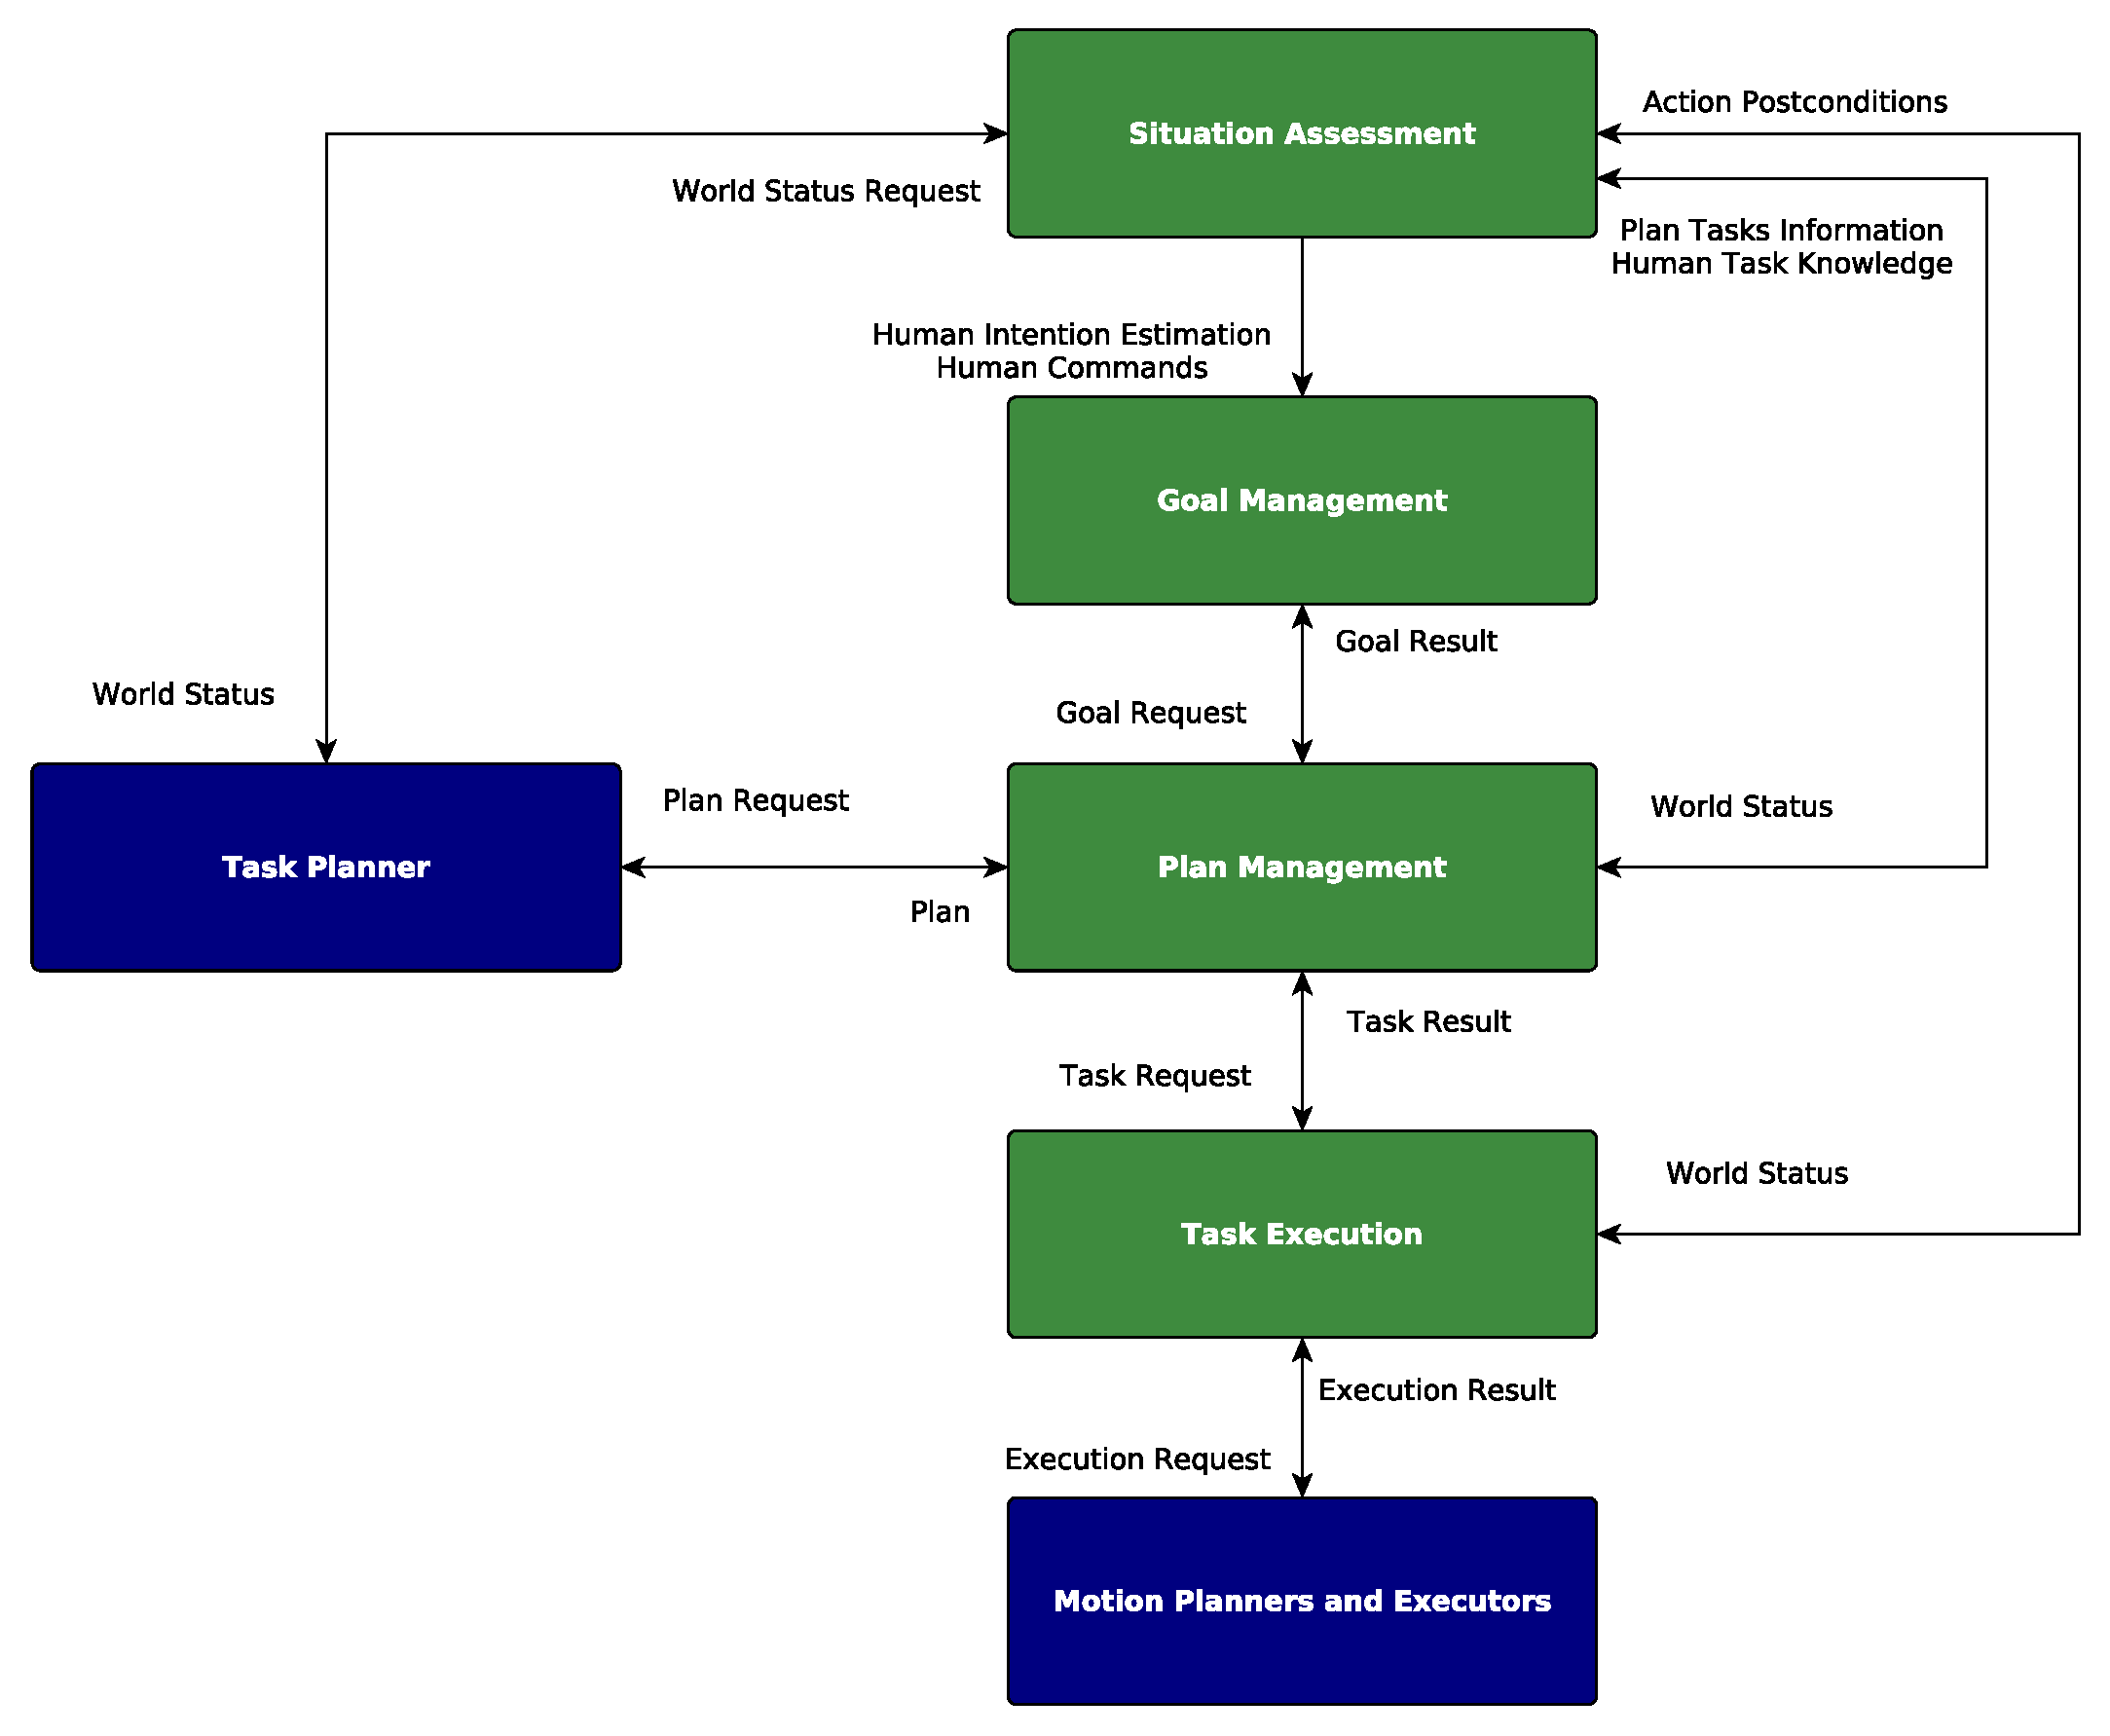
\includegraphics[scale=0.45]{img/intro/system_architecture.pdf}
	\caption[System architecture]{This picture shows the different layers of the system.}
	\label{fig:intro-system_architecture}
\end{figure}

The system also easily interface with different modules, which can be changed depending on the current needs:
\begin{itemize}
\item Task Planner. The Plan Production and Management layer provides an interface for different planners. New planners can be introduced by creating a bridge that respects the interface provided by the provided interface.
\item Motion Planners and Executors. The Execution Management layers is interfaced with a set of motion planners and an executor to accomplish the robot's movements and actions. New modules can be introduced by respecting the interface used in the layer.
\end{itemize}

\section{Organization of the Thesis}
This thesis is organized in several chapters. \ref{chapter:situation_assessment} discusses the Situation Assessment Layer, introducing its functionalities and a study to assess a part of its capacities. \ref{chapter:goal_management} shows how our system is able to receive, generate, and manage goals. \ref{chapter:plan_management} analyzes the capacity of our system to produce and manage plans. We discuss two different planners introduced in our system, and the process to explain, negotiate, and adapt plans to users. Finally, we present several plan management algorithms, with different characteristics. \ref{chapter:plan_execution} shows how our system is able to support action executed single-handedly by the robot, as well as our framework to execute joint actions with a human partner. \ref{chapter:case_study} presents two different applications where we used our system: a domestic robot helper and an airport guide. Finally, "introduce conclusion", concludes this work, discussing several possible future extensions. 

\section{Published Works}
\begin{itemize}
\item Milliez, Grégoire, et al. ``Simulating human-robot interactions for dialogue strategy learning." Simulation, Modeling, and Programming for Autonomous Robots. Springer International Publishing, 2014. 62-73.
\item Triebel, Rudolph, et al. ``SPENCER: A socially aware service robot for passenger guidance and help in busy airports.", 2015.
\item Fiore, Michelangelo, et al. ``An Adaptive and Proactive Human-Aware Robot Guide." Social Robotics. Springer International Publishing, 2015. 194-203.
\item Fiore Michelangelo, et al. ``On planning and task achievement modalities for human-robot collaboration." Experimental Robotics. Springer International Publishing, 2016.
\item Milliez, Grégoire, et al. ``Using human knowledge awareness to adapt collaborative plan generation, explanation and monitoring." The Eleventh ACM/IEEE International Conference on Human Robot Interation. IEEE Press, 2016.
\item Devin, Sandra et al. ``Some essential skills and their combination in an architecture for a cognitive and interactive" robot arXiv preprint arXiv:1603.00583, 2016
\item Caccavale, Riccardo, et al. ``Attentional Supervision of Human-Robot Collaborative Plans." The IEEE International Symposium on Robot and Human Interactive Communication (RO-MAN), 2016.
\end{itemize}